%; whizzy chapter -dvi
% -initex iniptex -latex platex -format platex -bibtex jbibtex -fmt fmt
% 以上 whizzytex を使用する場合の設定。

%     Tokyo Debian Meeting resources
%     Copyright (C) 2012 Junichi Uekawa
%     Copyright (C) 2011, 2015 Nobuhiro Iwamatsu

%     This program is free software; you can redistribute it and/or modify
%     it under the terms of the GNU General Public License as published by
%     the Free Software Foundation; either version 2 of the License, or
%     (at your option) any later version.

%     This program is distributed in the hope that it will be useful,
%     but WITHOUT ANY WARRANTY; without even the implied warranty of
%     MERCHANTABILITY or FITNESS FOR A PARTICULAR PURPOSE.  See the
%     GNU General Public License for more details.

%     You should have received a copy of the GNU General Public License
%     along with this program; if not, write to the Free Software
%     Foundation, Inc., 51 Franklin St, Fifth Floor, Boston, MA  02110-1301 USA

%  preview (shell-command (concat "evince " (replace-regexp-in-string "tex$" "pdf"(buffer-file-name)) "&"))

%%ここからヘッダ開始。

\documentclass[mingoth,a4paper]{jsarticle}
\usepackage{monthlyreport}
% 日付を定義する、毎月変わります。
\newcommand{\debmtgyear}{2020}
\newcommand{\debmtgmonth}{4}
\newcommand{\debmtgdate}{18}
% started from zero:
% (let ((year 2013) (month 7)) (+ (* (- year 2005) 12) month -1))
\newcommand{\debmtgnumber}{184}

% Needed to import pandoc-generated LaTeX documents.
% See https://stackoverflow.com/questions/40438037/tightlist-error-using-pandoc-with-markdown
\providecommand{\tightlist}{%
  \setlength{\itemsep}{0pt}\setlength{\parskip}{0pt}}

\begin{document}

\begin{titlepage}
\thispagestyle{empty}
% タイトルページ:編集必要な部分は最初のマクロに飛ばすこと

\vspace*{-2cm}
第\debmtgnumber{}回 東京エリア Debian 勉強会資料\\
\hspace*{-2cm}

\includegraphics{image2012-natsu/dotdeb.pdf}\\
\hfill{}\debmtgyear{}年\debmtgmonth{}月\debmtgdate{}日

% ここはアップデートすること
% 全角文字にしないとフォントのサイズが合わないので注意
\rotatebox{10}{\fontsize{30}{30} {\gt Wireguard・Jitsi特集}}\\

\vspace*{-2cm}
\hfill{}
\includegraphics[height=6cm]{image200502/openlogo-nd.eps}
\end{titlepage}

\newpage

\begin{minipage}[b]{0.2\hsize}
 \definecolor{titleback}{gray}{0.9}
 \colorbox{titleback}{\rotatebox{90}{\fontsize{80}{80} {\gt デビアン勉強会} }}
\end{minipage}
\begin{minipage}[b]{0.8\hsize}
\hrule
\vspace{2mm}
\hrule
\begin{multicols}{2}
\tableofcontents
\end{multicols}
\vspace{2mm}
\hrule
\end{minipage}

\dancersection{最近のDebian関連のミーティング報告}{杉本 典充}

\subsection{2020年3月度 東京エリア・関西合同Debian勉強会}

2020年3月21日(土)に東京エリアDebian勉強会と関西Debian勉強会の合同でオンラインによるDebian勉強会を開催しました。参加者は15名でした。

オンラインで行うにあたりいくつかのビデオ会議システムを試験利用しながら進行しました。利用したビデオ会議システムはGoogleハングアウト、上川さんが独自に構築したストリーミング配信サーバ、Jitsiサーバでした。

前半はセミナー発表を行い、タイトル「動画配信環境をしらべてみた」として上川さんが発表しました。RTMPというストリーミング配信を行うプロトコルの説明、RTMPに対応したストリーミング配信サーバを動作させて勉強会の参加者はVLCやffplayコマンドでストリーミング配信を視聴することができました。またOBS StudioというRTMPを扱う便利なアプリケーションの紹介もあり、ストリーミング配信の仕組みを学ぶことができました。

後半はBoFを行い、議題「今回のビデオ会議システムの品質について、流行りのビデオ会議システムについて」として情報を持ち寄りつつ、勉強会当日に利用したビデオ会議システムや代替のビデオ会議システムについて情報共有を行いました。

BoFの議事録は以下URLで公開しています。

\begin{itemize}
\item \url{https://tokyodebian-team.pages.debian.net/2020-03_tokyodebian_bof.txt}
\end{itemize}


\dancersection{事前課題}{杉本 典充}

今回の事前課題は以下です。

\begin{enumerate}
\item Wireguard はご存じですか
\item Jitsi はご存じですか
\end{enumerate}

%この課題に対して提出いただいた内容は以下です。

\begin{multicols}{2}
{\small
\begin{prework}{ dictoss }
  \begin{enumerate}
  \item $BCN$i$J$$(B
  \item $B;H$C$?$3$H$,$"$k(B
  \end{enumerate}
\end{prework}

\begin{prework}{ yy\_y\_ja\_jp }
  \begin{enumerate}
  \item $BCN$i$J$$(B
  \item $B;H$C$?$3$H$,$"$k(B
  \end{enumerate}
\end{prework}

\begin{prework}{ koedoyoshida }
  \begin{enumerate}
  \item $BCN$C$F$$$k$,!";H$C$?$3$H$O$J$$(B
  \item $BCN$C$F$$$k$,!";H$C$?$3$H$O$J$$(B
  \end{enumerate}
\end{prework}

\begin{prework}{ uwabami }
  \begin{enumerate}
  \item $BCN$C$F$$$k$,!";H$C$?$3$H$O$J$$(B
  \item $BCN$C$F$$$k$,!";H$C$?$3$H$O$J$$(B
  \end{enumerate}
\end{prework}

\begin{prework}{ yosuke\_san }
  \begin{enumerate}
  \item $BCN$C$F$$$k$,!";H$C$?$3$H$O$J$$(B
  \item $BCN$C$F$$$k$,!";H$C$?$3$H$O$J$$(B
  \end{enumerate}
\end{prework}

\begin{prework}{ kare-zeri-123 }
  \begin{enumerate}
  \item $BCN$i$J$$(B
  \item $BCN$i$J$$(B
  \end{enumerate}
\end{prework}

\begin{prework}{ hatsanhat }
  \begin{enumerate}
  \item $BCN$i$J$$(B
  \item $BCN$C$F$$$k$,!";H$C$?$3$H$O$J$$(B
  \end{enumerate}
\end{prework}


\begin{prework}{ Kazuhiro NISHIYAMA (znz) }
  \begin{enumerate}
  \item $B;H$C$?$3$H$,$"$k(B
  \item $B;H$C$?$3$H$,$"$k(B
  \end{enumerate}
\end{prework}

\begin{prework}{ TANIGUCHI Takaki (takaki\_t) }
  \begin{enumerate}
  \item $BCN$C$F$$$k$,!";H$C$?$3$H$O$J$$(B
  \item $BCN$i$J$$(B
  \end{enumerate}
\end{prework}

\begin{prework}{ SHIMOYAMA Yoshihiro (kurokouji) }
  \begin{enumerate}
  \item $BCN$i$J$$(B
  \item $BCN$i$J$$(B
  \end{enumerate}
\end{prework}

\begin{prework}{ sato\_makoto }
  \begin{enumerate}
  \item $BCN$i$J$$(B
  \item $BCN$C$F$$$k$,!";H$C$?$3$H$O$J$$(B
  \end{enumerate}
\end{prework}

\begin{prework}{ fpond }
  \begin{enumerate}
  \item $BCN$i$J$$(B
  \item $BCN$i$J$$(B
  \end{enumerate}
\end{prework}

\begin{prework}{ su\_do }
  \begin{enumerate}
  \item $BCN$i$J$$(B
  \item $BCN$i$J$$(B
  \end{enumerate}
\end{prework}

\begin{prework}{ $B1]??<#(B (enoki) }
  \begin{enumerate}
  \item $BCN$C$F$$$k$,!";H$C$?$3$H$O$J$$(B
  \item $B;H$C$?$3$H$,$"$k(B
  \end{enumerate}
\end{prework}

\begin{prework}{ $B$5$H$&$H$b$N$j(B (totosan365) }
  \begin{enumerate}
  \item $BCN$C$F$$$k$,!";H$C$?$3$H$O$J$$(B
  \item $BCN$C$F$$$k$,!";H$C$?$3$H$O$J$$(B
  \end{enumerate}
\end{prework}

\begin{prework}{ zinrai }
  \begin{enumerate}
  \item $BCN$C$F$$$k$,!";H$C$?$3$H$O$J$$(B
  \item $BCN$i$J$$(B
  \end{enumerate}
\end{prework}

\begin{prework}{ ysaito }
  \begin{enumerate}
  \item $BCN$i$J$$(B
  \item $B;H$C$?$3$H$,$"$k(B
  \end{enumerate}
\end{prework}

\begin{prework}{ matoken }
  \begin{enumerate}
  \item $B;H$C$?$3$H$,$"$k(B
  \item $B;H$C$?$3$H$,$"$k(B
  \end{enumerate}
\end{prework}

\begin{prework}{ dancerj }
  \begin{enumerate}
  \item $BCN$i$J$$(B
  \item $B;H$C$?$3$H$,$"$k(B
  \end{enumerate}
\end{prework}

\begin{prework}{ ipv6waterstar }
  \begin{enumerate}
  \item $BCN$i$J$$(B
  \item $BCN$i$J$$(B
  \end{enumerate}
\end{prework}

\begin{prework}{ kozo2 }
  \begin{enumerate}
  \item $BCN$i$J$$(B
  \item $BCN$C$F$$$k$,!";H$C$?$3$H$O$J$$(B
  \end{enumerate}
\end{prework}

\begin{prework}{ lurdan }
  \begin{enumerate}
  \item $BCN$C$F$$$k$,!";H$C$?$3$H$O$J$$(B
  \item $B;H$C$?$3$H$,$"$k(B
  \end{enumerate}
\end{prework}

\begin{prework}{ NOKUBI Takatsugu (knok) }
  \begin{enumerate}
  \item $B;H$C$?$3$H$,$"$k(B
  \item $B;H$C$?$3$H$,$"$k(B
  \end{enumerate}
\end{prework}

\begin{prework}{ yuyhiraka }
  \begin{enumerate}
  \item $BCN$C$F$$$k$,!";H$C$?$3$H$O$J$$(B
  \item $BCN$i$J$$(B
  \end{enumerate}
\end{prework}

\begin{prework}{ $B$"(B (cpa119) }
  \begin{enumerate}
  \item $BCN$i$J$$(B
  \item $BCN$i$J$$(B
  \end{enumerate}
\end{prework}

\begin{prework}{ hichon }
  \begin{enumerate}
  \item $BCN$C$F$$$k$,!";H$C$?$3$H$O$J$$(B
  \item $BCN$C$F$$$k$,!";H$C$?$3$H$O$J$$(B
  \end{enumerate}
\end{prework}

}
\end{multicols}

%\dancersection{Debian Trivia Quiz}{username}
%
%Debianの昨今の話題についてのQuizです。
%
%今回の出題範囲は\url{debian-devel-announce@lists.debian.org} や \url{debian-news@lists.debian.org}などに投稿された内容からです。
%
%\begin{multicols}{2}
%%; whizzy-master ../debianmeetingresume201211.tex
% $B0J>e$N@_Dj$r$7$F$$$k$?$a!"$3$N%U%!%$%k$G(B M-x whizzytex $B$9$k$H!"(Bwhizzytex$B$,MxMQ$G$-$^$9!#(B
%

\santaku
{DebConf13 $B$N3+:ECO$H3+:EF|$O!)(B}
{$BF|K\!"El5~ET(B 6$B7n(B20$BF|(B}
{$B%K%+%i%0%"(B $B%^%J%0%"(B 7$B7n(B8-14$BF|(B}
{$B%9%$%9!"%t%)!<%^%k%-%e(B 8$B7n(B11-18$BF|(B}
{3}
{$B%K%+%i%0%"$O(BDebConf12$B$N3+:ECO$G$9!#(B
DebConf13$B$O%9%$%9$N%-%c%s%WCO$G3+:E$G$9!#(B
6/20$B$O3'$5$sM=Dj$r6u$1$F$*$-$^$7$g$&!#(B}

\santaku
{$B@$3&$N(BWeb$B%5!<%P$G:G$b?M5$$N$"$k(BLinux $B%G%#%9%H%j%S%e!<%7%g%s(B(W3Techs$BD4$Y(B)$B$O!)(B}
{CentOS}
{Debian}
{Ubuntu}
{B}
{\url{http://w3techs.com/technologies/history_details/os-linux}$B$K7k2L$N%0%i%U$,$"$j$^$9!#(B
$B8=:_(B Linux $B$r;HMQ$7$F$$$k(B web $B%5!<%P$N(B 32.9\% $B$,(B Debian $B$rMxMQ$7$F$*$j!"$=$N3d9g$O8=:_$bA}2C$rB3$1$F$$$k$=$&$G$9!#(B}

\santaku
{Debian $B%+!<%M%k%A!<%`$N%a%s%P!<$G$"$j!"(Bkernel.org $B$N(B 3.2.y $B0BDjHG7ONs$N%a%s%F%J$G$b$"$k(B Ben Hutchings $B$5$s$,<!4|(B Debian $B0BDjHG$H0l=o$K=P2Y$5$l$k(B Linux $B%+!<%M%k$K(B (3.2 $B7ONs$N(B mainline $B$K$OL5$$(B) $BDI2C5!G=$,Ek:\$5$l$kM=Dj$G$"$k$H=R$Y$F$$$^$9!#(B
$BB?$/$NDI2CE@$NCf$K4^$^$l$J$$$b$N$O2?!)(B}
{PREEMPT\_RT}
{Hyper-V guest drivers$B$N6/2=(B}
{ARM64/AArch64$B%"!<%-%F%/%A%c%5%]!<%H(B}
{C}
{Hyper-V guest drivers$B$O(Bmainline kernel$B$G(B3.2$B$K$b4^$^$l$F$$$^$9$,!"$h$j2~A1$5$l$?(B3.4$B$+$i$N=$@5$,F3F~$5$l$^$9!#(B
PREEMPT\_RT$B$O%O!<%I%j%"%k%?%$%`$r<B8=$9$k$?$a$N(BPatch$B!"(B
linux-image-rt-amd64 , linux-image-rt-686-pae $B$N(Bmetapackage$B$G;HMQ$G$-$^$9!#(B
$B?7$7$$(BARM 64$B%S%C%H%"!<%-%F%/%A%c%5%]!<%H$O(Bmainline kernel 3.7$B$+$i(B}

\santaku
{Wookey$B$5$s$,%"%J%&%s%9$7$?(Balpha$BHG$N(BDebian port arm64 image$B$O!)(B}
{Debian/Ubuntu port image}
{Debian/KFreeBSD port image}
{Debian/GnuHurd port image}
{A}
{self-bootstrapp(non x86)$BBP1~$H$N$3$H$G$9!#(B\url{http://wiki.debian.org/Arm64Port}$B$G%9%F!<%?%9$,3NG'$G$-$^$9!#(B}

\santaku
{700,000$BHVL\$N%P%0$,Js9p$5$l$?F|$rEv$F$k(B700000thBugContest$B$N7k2L$,=P$^$7$?!#$=$NM=A[F|$HJs9pF|$O!)(B}
{2012/12/12$B$rM=A[$7$?(BDavidPrevot}
{$BM=A[F|(B:2013/02/04$B!"Js9pF|(B:2013/02/14}
{$BM=A[F|(B:2013/02/07$B!"Js9pF|(B:2013/02/14}
{$BM=A[F|(B:2013/02/14$B!"Js9pF|(B:2013/02/07}
{C}
{$B:G$b6a$$(B2013/02/14$B$rM=A[$7$?(BChristian Perrier$B$5$s$,Ev$F$^$7$?!#7k2L$O(B\url{http://wiki.debian.org/700000thBugContest}$B$G8x3+$5$l$F$$$^$9!#(B
$B$^$?!"(B800,000/1,000,000$BHVL\$N%P%0$,Js9p$5$l$kF|$rEv$F$k%3%s%F%9%H(B\url{http://wiki.debian.org/800000thBugContest}$B$b3+:E$5$l$F$$$^$9!#(B}

\santaku
{master.debian.org$B$,?7$7$$5!3#$K0\9T$5$l$^$7$?!#$3$l$O2?$N%5!<%P$G$7$g$&$+(B $B!)(B}
{@debian.org$B$N%a!<%k%5!<%P(B}
{$B%Q%C%1!<%8$N%^%9%?!<%5!<%P(B}
{$B%Q%C%1!<%8$N%9%]%s%5!<(B(mentor)$B$rC5$9%5!<%P(B}
{A}
{$B8E$$%5!<%P$O%G%#%9%/>c32Ey$,$"$C$?$N$G!"<wL?$HH=CG$5$l!"%G!<%?$,B;<:$9$kA0$K?7$7$$%5!<%P$K0\9T$5$l$^$7$?!#(Bftp-master.debian.org$B$O(BDebian$B$N(B official package $B%j%]%8%H%j$G$9!#%Q%C%1!<%8$N%9%]%s%5!<(B(mentor)$B$rC5$9$N$O(Bmentors.debian.net$B!#(B }

\santaku
{pbuilder$B$K(Bclang support$B$,DI2C$5$l$^$7$?!#C/$,=q$$$?%Q%C%A$G$7$g$&$+!)(B}
{Sylvestre Ledru}
{Junichi Uekawa}
{Hideki Yamane}
{C}
{Debian$B$N(BClang$B%5%]!<%H$OCe!9$H?J$s$G$$$^$9!#(B}

\santaku
{DPN - 2013$BG/(B3$B7n(B4$BF|9f$K<h$j>e$2$i$l$?F|K\$N%$%Y%s%H$O(B}
{Open Source Conference 2013 Tokyo/Spring}
{Open Source Conference 2013 Hamamatu}
{Open Source Conference 2013 Tokushima}
{A}
{\url{http://henrich-on-debian.blogspot.jp/2013/02/open-source-conference-2013-tokyospring.html} $B>\:Y$O8e$[$I!#(B}


%\end{multicols}


% % (query-replace-regexp "<.*?>" "")
% % (query-replace-regexp "^[    ]\+" "")

%-------------------------------------------------------------------------------
\dancersection{Jitsiを使ったビデオ会議サーバの作り方}{杉本 典充}
%-------------------------------------------------------------------------------

\subsection{はじめに}

Debian Project は開発や開発者同士のコミュニケーションをオンライン上で行うことを前提として作業を進めています。ただ、開発者同士のオフラインによる繋がりを定期的に持ってもいいのではないかという考えから東京エリア Debian 勉強会が 2005 年に始まりました。

しかし、2019 年の年末あたりから流行し始めた新型コロナウイルス(COVID-19)の感染拡大を抑えるには人との接触をいかに回避できるかが重要になっています。そのため、直接人と会わずにコミュニケーションをとることができるビデオ会議のニーズが急激に高まってきています。

Debian 勉強会を含めたコンピュータの勉強会は以前から活発に行われていますが集会スタイルで行うことが多かったため、従来のやり方では開催が困難になっている実態があります。

そこで Debian 勉強会をオンラインで開催する手法としてビデオ会議システムをオープンソースで構築できる Jitsi(ジッチー)というサーバアプリケーションを試しているためご紹介します。


\subsection{Jitsiについて}

Jitsi\footnote{\url{https://jitsi.org/}}とは「More secure, more flexible, and completely free video conferencing」と謳うオープンソースなビデオ会議サーバの機能をもつアプリケーションです。Jitsi は ビデオ会議の機能を実現するために WebRTC の技術を利用しており、多くの PC ではグラフィカルな Web ブラウザを使ってビデオ会議を行うことができます。また、モバイル向けに Android 版および iOS 版のアプリケーションも存在します。

Jitsi のソースコードは github\footnote{\url{https://github.com/jitsi}}で公開しており、Java・Lua・html・javascriptを利用して開発しています。

ビデオ会議システムのセキュリティは大丈夫であるか、という疑問に対してJitsiはセキュリティとプライバシーについて以下のように説明しています\footnote{\url{https://jitsi.org/blog/security/}}。

\begin{itemize}
\item 会議室は最初の一人がログインしたタイミングで生成し、全員が退出すると会議室は破棄する設計である
  \begin{itemize}
  \item 全員が退出した後は名前、電子メールアドレス、プロフィール写真は保持されない
  \item 全員が退出した後に同名の会議室に入った場合は以前の同名の会議室とは別扱いになり、データを引き継がない
  \end{itemize}
\item ビデオ会議のビデオおよびオーディオのストリーミングデータはは DTLS-SRTP\footnote{\url{https://tools.ietf.org/html/rfc5763}}を用いて暗号化した上で通信を行う
  \begin{itemize}
  \item パケットの暗号化及び復号は会議の参加者が2人の場合は参加者のデバイス同士が直接処理し、3人以上の場合はJitsi Videobridge (JVB) が中継して復号と変換処理を行う方式をとっている
  \item ネットワークのトラフィックはメモリのみ存在し、永続ストレージに保存されることはない
  \end{itemize}
\item モデレータの権限をもつユーザは、指定したユーザへ「キック(退出)」「ミュート(音量ゼロ)」を実行できる
\item 会議室名はできるだけランダムな長い名前にすることが望ましい
  \begin{itemize}
  \item よくある単語名や名詞を会議室名に使うと常に誰か会議室にいる状態になり、会議室が破棄されなくなるため
  \end{itemize}
\end{itemize}


\subsection{Jitsiサーバの作り方}

\subsubsubsection{Jitsiのインストール情報}

Jitsi のインストール情報は以下のページで紹介しています。今回はこの手順を参考にサーバを構築しています。

\begin{itemize}
\item 公式情報
  \begin{itemize}
  \item \url{https://github.com/jitsi/jitsi-meet/blob/master/doc/quick-install.md}
  \item \url{https://github.com/jitsi/docker-jitsi-meet} \\ NAT が必要なサーバで動作する設定、クライアント・サーバの通信で利用するポート番号の説明があります
  \end{itemize}
\item Debian 10 Buster に Jitsiをインストールした方の情報
  \begin{itemize}
  \item \url{https://www.scaleway.com/en/docs/setting-up-jitsi-meet-videoconferencing-on-debian-buster/}
  \end{itemize}
\end{itemize}


\subsubsection{DNS名の事前決定}

Jitsi サーバをグローバル環境、またはイントラネットのどちらで環境を構築する場合でも DNS 名を先に決めておくことをお勧めします。

理由は Jitsi の debianパッケージをインストールする過程で DNS 名を入力するダイアログが表示され、実際に利用するDNS名を入力しておくとインストール後のファイル名や通信設定の大部分が自動で設定されるためかなり楽ができます。

今回は、DNS名を "vc2.pcdennokan.wjg.jp" としてグローバル環境にサーバを構築する前提とします。なお、DNS サーバはダイナミック DNS の サービスである MyDNS.JP\footnote{\url{https://www.mydns.jp/}}を利用しています。


\subsubsection{サーバの準備}

Jitsi サーバは以下の条件を満たす性能及び場所に作成するのがよいと考えます。

\begin{itemize}
\item RAMは4GB以上が望ましい(デフォルト状態でのjavaプロセスの起動オプションに"-Xmx3072m"\footnote{/usr/share/jitsi-videobridge/lib/videobridge.rc に "\# VIDEOBRIDGE\_MAX\_MEMORY=3072m" というパラメータがあります。}を指定しており、JavaのOut of Memoryエラーが発生しにくい)
\item インターネット回線の容量が大きく、できればトラフィックの単価が安いサーバやサービスを使う(ストリーミングを行うためネットワークのトラフィック量がかなり激しい)
\item ビデオ会議の同時利用人数が多い場合はCPUコア数が多い方がよい(同時利用人数が多いとロードアベレージが上がる傾向がある)
\item ディスク I/O はほとんどないアプリケーションをインストールする分の容量があればよい
\end{itemize}

今回は作成する Jitsi サーバは以下の環境で用意しました。

\begin{itemize}
\item クラウドサービス
  \begin{itemize}
  \item Google Compute Engine (GCE)
  \end{itemize}
\item サーバのスペック
  \begin{itemize}
  \item マシンタイプ: N1 ハイ CPU マシンタイプ n1-highcpu-4
  \item vCPU: 4 コア
  \item RAM: 3.60 GB
  \item ネットワーク下り帯域幅: 10 Gbps
  \item Disk: 10 GB
  \item OS: Debian 10.3 Stretch
  \end{itemize}
\end{itemize}

GCE で仮想サーバを作成するときに http と https の通信を許可する設定のチェックボックスを有効にしておきます。


\subsubsection{ファイアウォール}

Jitsi サーバで通信を行うためにファイアウォールを設定して必要な通信を許可する必要があります。

PC やモバイルアプリでビデオ会議を行う場合は以下のポート番号の通信を許可してください。

\begin{itemize}
\item 80/tcp
\item 443/tcp
\item 10000/udp
\end{itemize}

クライアントPC と Jitsi サーバが通信する構成は以下のURLの図がわかりやすいと思います。

\url{https://github.com/jitsi/docker-jitsi-meet#architecture}


\subsubsection{サーバへのログイン}

手元の Debian 上から GCE の仮想サーバを ssh で操作するには、Google Cloud SDK のインストールが必要です。次の URL の手順に従い "google-cloud-sdk" パッケージをインストールしておいてください。

\begin{itemize}
\item \url{https://cloud.google.com/sdk/docs/downloads-apt-get?hl=ja}
\end{itemize}

google-cloud-sdk パッケージをインストールして認証情報の設定が完了後、以下のコマンドを実行すると ssh で仮想サーバにログインできます。

\begin{commandline}
$ gcloud compute ssh videochat2 --zone asia-northeast1-c --ssh-flag="-p 22"
\end{commandline}


\subsubsection{Debianサーバの初期セットアップ}

GCE で用意している Debian 10.3 buster のイメージはタイムゾーンは UTC、ロケールは C が初期値になっています。日本語環境で利用するため、設定を変更します。

\subsubsubsection{タイムゾーンの変更}

現在のタイムゾーンを確認します。

\begin{commandline}
$ date
Sun Apr 12 02:22:51 UTC 2020
\end{commandline}

タイムゾーンを変更するには、dpkg-reconfigure コマンドで設定します。

\begin{commandline}
$ sudo dpkg-reconfigure tzdata
  → Asia を選択
  → Tokyo を選択

Current default time zone: 'Asia/Tokyo'
Local time is now:      Sun Apr 12 11:23:20 JST 2020.
Universal Time is now:  Sun Apr 12 02:23:20 UTC 2020.
\end{commandline}

タイムゾーンが変更されたことを確認します。

\begin{commandline}
$ date
Sat Apr 18 00:21:56 JST 2020
\end{commandline}


\subsubsubsection{ロケール}

日本語のロケールを使用するには locales パッケージをインストールし、dpkg-reconfigure コマンドで設定します。

\begin{commandline}
$ sudo apt-get update
$ sudo apt-get install locales
$ sudo dpkg-reconfigure locales
  → Configuring locales
    → ja_JP.UTF-8 を選択
  → Default locale for the system environment
    → ja_JP.UTF-8 を選択
\end{commandline}


\subsubsubsection{サーバの再起動と動作確認}

サーバを再起動してタイムゾーンとロケールの変更を全プロセスに反映させます。

\begin{commandline}
$ sudo reboot
\end{commandline}

タイムゾーンとロケールの状態を確認します。

\begin{commandline}
$ date
2020年  4月 18日 土曜日 00:30:38 JST
\end{commandline}


\subsubsubsection{NTPサーバの確認}

GCE では NTPサーバとして chronyd が 標準で動作しています。

\begin{commandline}
$ ps ax | grep chrony | grep -v grep
  365 ?        S      0:00 /usr/sbin/chronyd -F -1
  366 ?        S      0:00 /usr/sbin/chronyd -F -1
\end{commandline}


\subsubsection{Jitsiのインストール}

\subsubsubsection{nginxのインストール}

Jitsi サーバとクライアント PC の通信は直接 jitsi-videobridge2 デーモンと行うか、リバースプロキシを経由して jitsi-videobridge2 と通信するかのどちらを選択できます。今回はリバースプロキシを経由することとし、 nginx を利用します。apt-get コマンドで nginx をインストールします。

\begin{commandline}
$ sudo apt-get install nginx
$ sudo systemctl start nginx
$ sudo systemctl enable nginx
\end{commandline}

重要なポイントは後述する jitsi-meet パッケージをインストールするより前に nginx をインストールしておくことです。jitsi-meet パッケージはインストール処理で設定ファイルを生成するのですが、 web サーバがインストール済みの場合はリバースプロキシで動作することを前提とした設定ファイルを自動で生成するようです\footnote{\url{https://www.scaleway.com/en/docs/setting-up-jitsi-meet-videoconferencing-on-debian-buster/}}。


\subsubsubsection{Jitsiのインストール}

Jitsi のインストールで利用するコマンドをインストールます。

\begin{commandline}
$ sudo apt-get install wget
\end{commandline}

Jitsi で用意している apt リポジトリを登録します。残念ながら jitsi のパッケージは debian の公式パッケージとして stable 版、unstable 版ともに提供されていません。

\begin{commandline}
$ wget -qO - https://download.jitsi.org/jitsi-key.gpg.key | sudo apt-key add -
$ sudo sh -c "echo 'deb https://download.jitsi.org stable/' > /etc/apt/sources.list.d/jitsi-stable.list"
$ sudo apt-get update
\end{commandline}

jitsi-meetパッケージをインストールします。

\begin{commandline}
$ sudo apt-get install jitsi-meet
\end{commandline}

jitsi-meet パッケージのインストール時に DNS 名を入力するダイアログが表示されますので、決めておいた DNS 名を入力します。また、SSL証明書をどうするか質問するダイアログも続けて表示されます。これは「Generate a new self-signed certificate (You will later...」を選択してインストールを行います(後述の手順で Let's Encrypt の SSL 証明書をインストールします)。

jitsi-meet をインストールすると、2020年4月10日にリリースされた以下のパッケージがインストールされました。

\begin{commandline}
norimitu@videochat2:~$ dpkg -l | grep jitsi
ii  jitsi-meet             2.0.4416-1           all  WebRTC JavaScript video conferences
ii  jitsi-meet-prosody     1.0.3992-1           all  Prosody configuration for Jitsi Meet
ii  jitsi-meet-turnserver  1.0.3992-1           all  Configures coturn to be used with Jitsi Meet
ii  jitsi-meet-web         1.0.3992-1           all  WebRTC JavaScript video conferences
ii  jitsi-meet-web-config  1.0.3992-1           all  Configuration for web serving of Jitsi Meet
ii  jitsi-videobridge2     2.1-169-ga28eb88e-1  all  WebRTC compatible Selective Forwarding Unit (SFU)
\end{commandline}


\subsubsubsection{Let's EncryptのSSL証明書のインストール}

jitsi-meet パッケージのインストール時に自己署名証明書を生成していますが、ターミナルの出力の中に Let's Encrypt の SSL 証明書を簡単にインストールするスクリプトがあるというメッセージが表示されています。

以下のコマンドを実行して Let's Encrypt の SSL 証明書をインストールします\footnote{DNSのAレコードが事前に登録されていない場合は Let's Encrypt の SSL 証明書の取得処理がエラーになりますのでご注意ください。}。

\begin{commandline}
$ sudo bash /usr/share/jitsi-meet/scripts/install-letsencrypt-cert.sh
\end{commandline}

ここまでインストール作業を終えて webブラウザで https://vc2.pcdennokan.wjg.jp/ へ接続すると Jitsi のトップ画面(図 \ref{fig:jitsi-web-top})を表示できます。

\begin{figure}[h]
\begin{center}
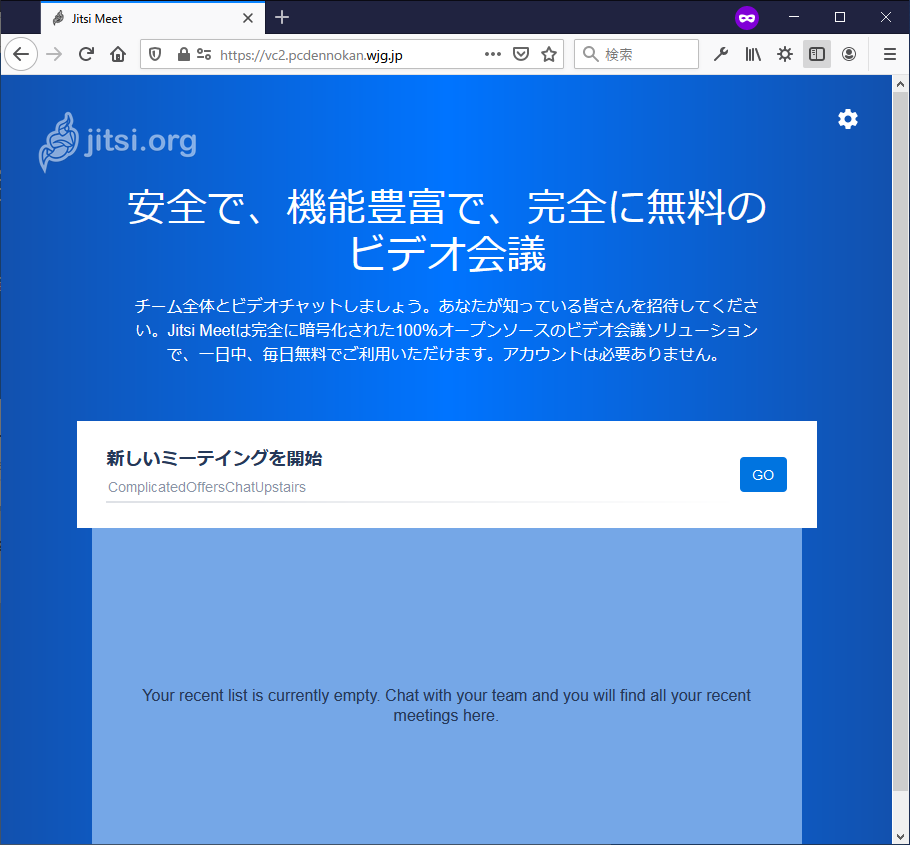
\includegraphics[keepaspectratio,width=0.6\hsize]{image202004/jitsi_web_top.png}
\end{center}
\caption{Jitsiサーバのwebのトップ画面}
\label{fig:jitsi-web-top}
\end{figure}


\subsubsubsection{(オプション設定)NAT 環境の後ろで Jitsi サーバを動かす設定}

Jitsi サーバを置くネットワーク構成によっては、サーバがグローバル IP アドレスを直接持たず NAT してインターネットに接続する構成の場合があります(GCE や Docker を利用する場合は NAT 構成になります)。その場合は jitsi-videobridge2 デーモンに設定を加える必要があります\footnote{イントラネット環境やグローバルIPを直接サーバに割り当てるネットワーク構成の場合はこの設定変更は不要です。}。

\begin{commandline}
$ sudo vi /etc/jitsi/videobridge/sip-communicator.properties
    (snip)
org.ice4j.ice.harvest.NAT_HARVESTER_LOCAL_ADDRESS=10.146.0.6
org.ice4j.ice.harvest.NAT_HARVESTER_PUBLIC_ADDRESS=34.84.236.29
    (snip)
\end{commandline}

jitsi-videobridge2 デーモンを再起動して設定を反映します。

\begin{commandline}
$ sudo systemctl restart jitsi-videobridge2
\end{commandline}

NAT設定の説明は以下 URL に情報があります。

\url{https://github.com/jitsi/jitsi-meet/blob/master/doc/quick-install.md#advanced-configuration}


\subsubsection{ビデオ会議を行う}

ここまで設定してようやく Jitsi を使ってビデオ会議ができるようになりました。

以下のURLへアクセスし、画面中央の「新しいミーティングを開始」に会議室名を入力するとビデオ会議のURLへジャンプして会議室ができます。会議に参加する方にはそのURLを連絡し、WebブラウザまたはモバイルアプリでURLを開くことで会議に参加することができます。

\begin{itemize}
\item https://vc2.pcdennokan.wjg.jp/
\end{itemize}


\subsection{Jitsiのカスタマイズについて}

\subsubsection{設定ファイルの場所}

Jitsi の設定ファイルは "/etc/jitsi" 配下及び "/usr/share/jitsi-*" 配下のディレクトリにあります。主な設定ファイルを以下に示します。

\begin{itemize}
\item /etc/jitsi/meet/vc2.pcdennokan.wjg.jp-config.js \\(インストール時に入力したDNS名を含むファイル名が生成されます)
\item /usr/share/jitsi-meet/interface\_config.js
\item /usr/share/jitsi-meet/libs/external\_api.min.js
\end{itemize}


\subsubsection{最近の会議室一覧の非表示}

Jitsi のトップ画面を開くと最近作成された会議室の一覧が表示されます。ただ、会議室の存在を知る人を制限するには誰でも会議室の URL がわかる状態になっているのは好ましくありません。

/usr/share/jitsi-meet/interface\_config.js の "RECENT\_LIST\_ENABLED" パラメータを変更すると Jitsi の最近の会議室一覧の表示をしないようにできます。

\begin{commandline}
# vi /usr/share/jitsi-meet/interface_config.js
  (snip)
  
  RECENT_LIST_ENABLED: false,

  (snip)
\end{commandline}


\subsubsection{ストリーミングのビデオの画質調整}

Jitsi のビデオ会議の画質はサーバ側で HD(720p、1280x720px)がデフォルトに設定されています\footnote{ノートPCに搭載しているWebカメラのほとんどはHD(720p、1280x720px)の品質のものが多いです。}。大変きれいなのですが、パケットの転送量が多くなるため通信帯域が細い場合に遅延が起こる、クライアントPCとJitsiサーバの負荷が高くなる、Jitsi サーバのトラフィックにかかる料金が気になる、などストリーミングならではの悩みが出てきます。

config.js の設定変更を行うとビデオ会議の画質を変更することができます。"resolution" 値はクライアント PC の Web カメラの解像度の設定値であり、"constraints" のオブジェクトの値はクライアント PC が視聴する他の参加者のビデオの画質の設定値です。

以下の config.js はクライアント PC の Web カメラの解像度の画質を「480p」とし、クライアント PC が視聴する他の参加者のビデオの画質を「480p〜240p」とする設定例です。

\begin{commandline}
# vi /etc/jitsi/meet/vc2.pcdennokan.wjg.jp-config.js
    (snip)
  
   // Sets the preferred resolution (height) for local video. Defaults to 720.
    resolution: 480,

    // w3c spec-compliant video constraints to use for video capture. Currently
    // used by browsers that return true from lib-jitsi-meet's
    // util#browser#usesNewGumFlow. The constraints are independent from
    // this config's resolution value. Defaults to requesting an ideal
    // resolution of 720p.
    constraints: {
        video: {
            height: {
                ideal: 480,
                max: 480,
                min: 240
            }
        }
    },

    (snip)
\end{commandline}

なお config.js は https://vc2.pcdennokan.wjg.jp/config.js のURLでクライアント PC へ配信されます。


\subsection{2020年3月Debian勉強会のJitsiサーバのリソース使用量}

\subsubsection{サーバ環境}

2020 年 3 月に開催したDebian 勉強会の後半は Jitsi サーバを試験的に利用して 15 名で BoF を 1 時間程度行いました。その時のサーバ環境、サーバリソースの使用量を公開します。

Jitsi サーバは以下の環境で用意していました。

\begin{itemize}
\item クラウドサービス
  \begin{itemize}
  \item Google Compute Engine (GCE)
  \end{itemize}
\item サーバのスペック
  \begin{itemize}
  \item マシンタイプ: N1 標準マシンタイプ n1-standard-1
  \item vCPU: 1 コア
  \item RAM: 3.75 GB
  \item ネットワーク下り帯域幅: 2 Gbps
  \item Disk: 10 GB
  \item OS: Debian 9 Stretch\footnote{Webの情報ではDebian 9のインストール情報が多く見つかり、時間的制約からDebian 9を選んだ経緯があります。}
  \end{itemize}
\end{itemize}

Jitsiアプリケーションのバージョンは以下でした(2020 年 4 月 18 日現在の最新版より少し古いバージョンです)。

\begin{commandline}
$ dpkg -l | grep jitsi
ii  jitsi-meet             1.0.4101-1  all    WebRTC JavaScript video conferences
ii  jitsi-meet-prosody     1.0.3729-1  all    Prosody configuration for Jitsi Meet
ii  jitsi-meet-web         1.0.3729-1  all    WebRTC JavaScript video conferences
ii  jitsi-meet-web-config  1.0.3729-1  all    Configuration for web serving of Jitsi Meet
ii  jitsi-videobridge      1126-1      amd64  WebRTC compatible Selective Forwarding Unit (SFU)
\end{commandline}


\subsubsection{CPU利用率}

サーバの CPU 利用率のグラフを 図 \ref{fig:graph_jitsi-cpu-usage} に示します。ピーク時で 86\%の使用率でした。CPU コア数は 1 コアの割り当てのため、意外と処理できていた感じがあります。

なお、当日サーバ上で top コマンドの表示を確認していたときはのロードアベレージが 6 程度だった記憶があります。

\begin{figure}[h]
\begin{center}
  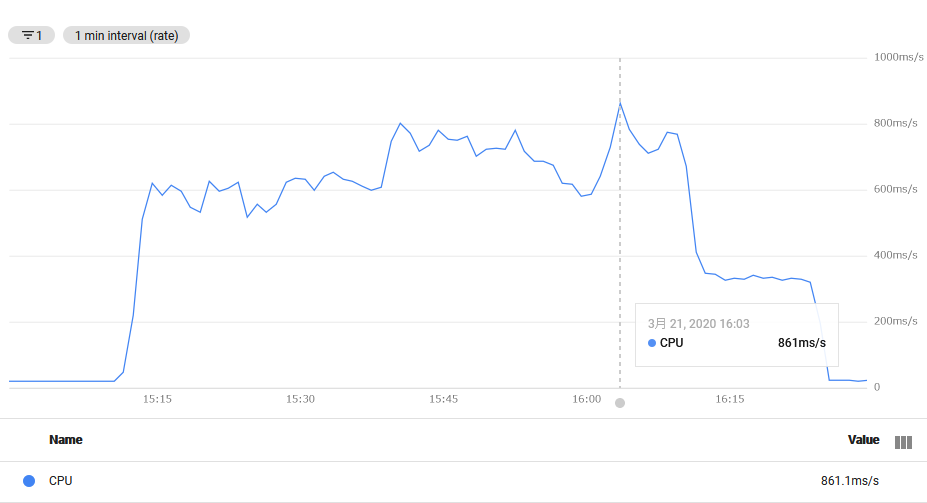
\includegraphics[keepaspectratio,width=0.75\hsize]{image202004/jitsi_perf_cpu_usage.png}
\end{center}
\caption{JitsiサーバのCPU利用率のグラフ(vCPU割り当て数:1)}
\label{fig:graph_jitsi-cpu-usage}
\end{figure}


\subsubsection{受信トラフィック}

サーバの受信(上り)トラフィックのグラフを 図 \ref{fig:graph_jitsi-traffic-recv} に示します。ピーク時で 1.653 MiB/s(= 13.22 Mbps) の受信トラフィックがあり、15 台のクライアントPCから受信したストリーミングデータの合計値となります。ただ、参加者は利用するクライアント PC の Web カメラを無効にしていた方が多く音声データのみを送信している人が多かったと推測しています。

\begin{figure}[h]
\begin{center}
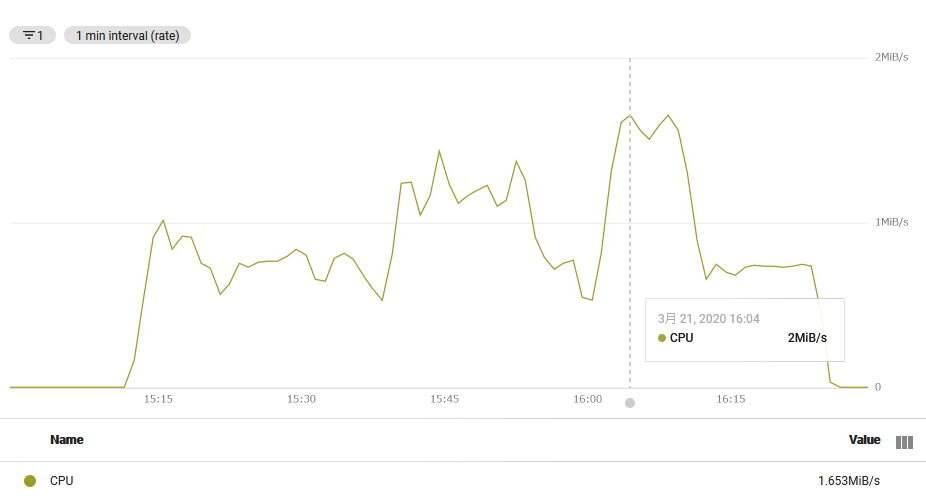
\includegraphics[keepaspectratio,width=0.75\hsize]{image202004/jitsi_perf_nw_recv-byte.png}
\end{center}
\caption{Jitsiサーバの受信トラフィックのグラフ}
\label{fig:graph_jitsi-traffic-recv}
\end{figure}


\subsubsection{送信トラフィック}

サーバの送信(下り)トラフィックのグラフを 図 \ref{fig:graph_jitsi-traffic-send} 示します。ピーク時で 6.828 MiB/s(= 54.62 Mbps) の送信トラフィックがあり、15 台のクライアント PC へ送信したストリーミングデータの合計値となります。会議の参加者の目線で見ると、参加者が利用するクライアント PC の Web カメラを無効にしていた方が多かった状態でピーク時に一人あたり 3.66 Mbps の受信トラフィックが出ていた計算となります。

仮に会議中に 55 Mbps の送信トラフィックが常に出ていると仮定するした場合、1 GB の送信トラフィックを 2 分 30 秒で消費します。120 分の勉強会で利用した場合は約 48 GB の送信トラフィックが発生する計算になります。

\begin{figure}[h]
\begin{center}
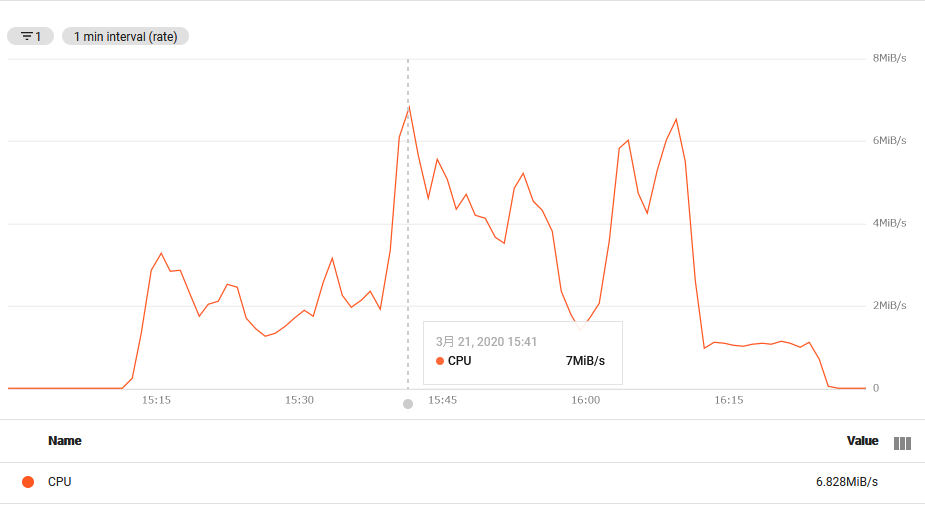
\includegraphics[keepaspectratio,width=0.75\hsize]{image202004/jitsi_perf_nw_send-byte.png}
\end{center}
\caption{Jitsiサーバの送信トラフィックのグラフ}
\label{fig:graph_jitsi-traffic-send}
\end{figure}


\subsubsection{おわりに}

Jitsi サーバを実際に構築してオンラインのビデオ会議で使ってみました。Jitsi サーバの快適な動作に必要なサーバ性能やネットワーク帯域はクライアントPCのカメラの解像度やフレームレートによっても変わってきます。自分好みの設定に調整できること、イントラネットに自分でビデオ会議サーバを作れること、そしてソースコードの書き換えもできること、これがオープンソースの醍醐味ですのでぜひとも Jitsi を利用してみてください。


% 冊子にするために、4の倍数にする必要がある。
% そのための調整
\dancersection{メモ}{}
\mbox{}\newpage

\vspace*{15cm}
\hrule
\vspace{2mm}

\includegraphics[width=2cm]{image200502/openlogo-nd.eps}
\noindent \Large \bf Debian 勉強会資料\\
\noindent \normalfont \debmtgyear{}年\debmtgmonth{}月\debmtgdate{}日 \hspace{5mm}  初版第1刷発行\\
\noindent \normalfont 東京エリア Debian 勉強会 (編集・印刷・発行)\\
\hrule

\end{document}
